\chapter{REST e Docker}

\section{REST}

\subsection{Introduzione}

\dfn{REST}{
	REST è uno stile architetturale per creare APIs in rete: specifica la forma e la semantica della comunicazione tra un provider (server) e un consumer (client).
}

\nt{REST sta per REpresentional State Transfer.}

\clm{}{}{
	\begin{itemize}
		\item Il provider fornisce \fancyglitter{risorse concettuali}.
		\item Il consumer può manipolare una risorsa scambiando sue rappresentazioni.
		\item Le interazioni avvengono mediante richieste \fancyglitter{stateless} con un interfaccia uniforme (HTTP, URI, etc.).
		\item Solitamente si implementa con HTTP (mappa naturalmente con i principi REST).
		\item Sia il provider che il consumer devono essere \fancyglitter{compliant} con la specifica API concordata.
	\end{itemize}
}

\cor{REST Resources}{
	Gli Endpoint URIs (pathname) dovrebbero esprimere risorse (nomi), non azioni. Mappano sui DDD:
	\begin{itemize}
		\item Part di path rappresentano entità (tipi + id).
		\item Path annidate rappresentano oggetti aggregati o contenuti.
	\end{itemize}
}

\begin{figure}[h]
	\centering
	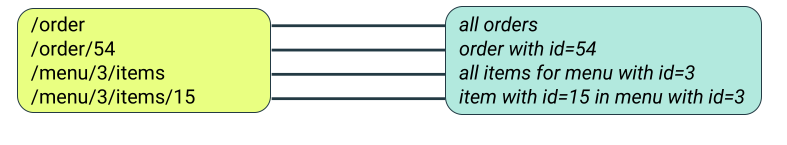
\includegraphics[scale=0.6]{02/rest res.png}
	\caption{Esempio di mappatura REST resources su DDD.}
\end{figure}

\subsection{Verbi e Status Responses}

\cor{REST Verb}{
	I verbi esprimono le azioni effettuate su una risorsa. I verbi di REST mappano su metodi HTTP.
}

\paragraph{I verbi:}

\begin{itemize}
	\item GET ottiene una rappresentazione di una risorsa specifica (legge dei dati):
	      \begin{itemize}
		      \item Non ha side effects ed è idempotente.
		      \item Non ha un body.
		      \item \fancyglitter{Query String:} usata per aggiungere filtri sulla richiesta.
	      \end{itemize}

	      \begin{figure}[h]
		      \centering
		      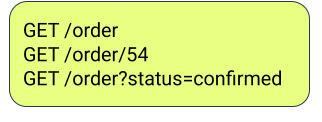
\includegraphics[scale=0.65]{02/GET.png}
		      \caption{REST GET.}
	      \end{figure}

	\item POST viene usata per creare una nuova risorsa:
	      \begin{itemize}
		      \item Ha side effects e non è idempotente.
		      \item Il body contiene la rappresentazione della nuova risorsa.
		      \item \fancyglitter{Query String:} usata per esprimere modificatori per la richiesta.

	      \end{itemize}

	      \begin{figure}[h]
		      \centering
		      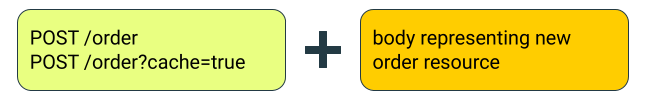
\includegraphics[scale=0.65]{02/POST.png}
		      \caption{REST POST.}
	      \end{figure}

	\item PUT rimpiazza una risorsa esistente con una nuova rappresentazione:
	      \begin{itemize}
		      \item Ha side effects, ma è idempotente.
		      \item Il body contiene una rappresentazione aggiornata della risorsa.
		      \item \fancyglitter{Query String:} usata per aggiungere filtri sulla richiesta (come in POST).

	      \end{itemize}

	      \begin{figure}[h]
		      \centering
		      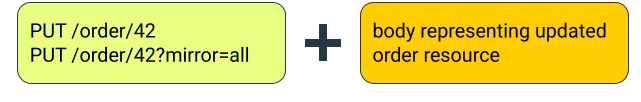
\includegraphics[scale=0.65]{02/PUT.png}
		      \caption{REST PUT.}
	      \end{figure}

	\item DELETE cancella una risorsa esistente:
	      \begin{itemize}
		      \item Ha side effects, ma è idempotente.
		      \item Non ha un body (come in GET).
		      \item \fancyglitter{Query String:} usata per aggiungere filtri sulla richiesta (come in POST).

	      \end{itemize}
	      \begin{figure}[h]
		      \centering
		      
\includegraphics[scale=0.65]{02/DELETE.png}
		      \caption{REST DELETE.}
	      \end{figure}


	\item PATCH aggiorna solo una parte della risorsa:
	      \begin{itemize}
		      \item Ha side effects, può essere idempotente o meno (dipende dal tipo di aggiornamento).
		      \item Il body contiene o una rappresentazione parziale delle risorse o i cambiamenti applicati.
		      \item \fancyglitter{Query String:} usata per aggiungere filtri sulla richiesta (come in POST).

	      \end{itemize}
	      \begin{figure}[h]
		      \centering
		      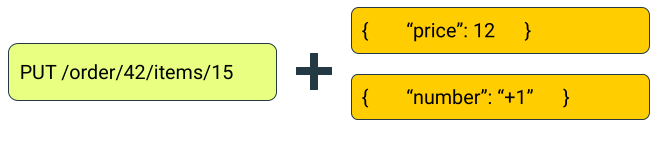
\includegraphics[scale=0.65]{02/PATCH.png}
		      \caption{REST DELETE.}
	      \end{figure}
\end{itemize}

\dfn{REST Status Responses}{

	REST associa specifici significati agli status code che devono essere rispettati per la compliance.
}

\paragraph{Risposte:}

\begin{itemize}
	\item 2XX - Successo:
	      \begin{itemize}
		      \item 200 - OK: successo generico.
		      \item 201 - Created: una POST che ha creato con successo una nuova risorsa.
		      \item 204 - No Content: operazione che ha avuto successo ma non ha restituito un body (DELETE o PUT).
	      \end{itemize}
	\item 3XX - Redirezione:
	      \begin{itemize}
		      \item 303 - See Other: dopo che una POST redirige a una GET della risorsa creata.
	      \end{itemize}
	\item 4XX - Errore Client:
	      \begin{itemize}
		      \item 400 - Bad Request: la richiesta è malformata.
		      \item 401 - Unauthorized: credenziali mancanti o invalide.
		      \item 403 - Forbidden: l'utente è autenticato, ma non è autorizzato ad accedere a tali risorse.
		      \item 404 - Not Found: la risorsa desiderata non esiste.
		      \item 409 - Conflict: lo stato attuale del sistema è in conflitto con l'operazione (per business rulles, etc.)
		      \item 422 - Unprocessable Entity: la richiesta viola delle regole semantiche.
		      \item 429 - Too Many Requests - superà il limite di richieste possibili\footnote{Indovinate chi è stata bannata dall'AUR per aver spammato richieste LOL.}.
	      \end{itemize}
	\item 5XX - Errore Server:
	      \begin{itemize}
		      \item 500 - Internal Server Error: eccezione generica.
		      \item 502 - Bad Gateway: il servizio fallisce per via di un fallimento upstream (proxies).
		      \item 503 - Service Unavailable: servizio temporaneamente down.
		      \item 504 - Gateway Timeout: timeout upstream (proxies).
	      \end{itemize}
\end{itemize}

\paragraph{REST vs. RPC:}

\begin{itemize}
	\item REST: gli endpoint identificano risorse, i verbi dicono cosa fare con essere e il body rappresenta la rappresentazione delle risorse.
	\item RPC: gli endpoint esprimono le operazioni da fae e il body rappresenta i parametri ( nella richiesta) o il valore restituito (nella risposta).
\end{itemize}

\paragraph{Pragmatic REST:}

\begin{itemize}
	\item Anche usando i verbi a volte è necessario che gli endpoint esprimano operazioni:
	      \begin{itemize}
		      \item Quando la semantica operazionale è a grana  troppo fine per essere limitata ai verbi.
		      \item Quando le operazioni non corrispondono a risorse esistenti nel server.
	      \end{itemize}
	\item Si può provare a rimanere REST:
	      \begin{itemize}
		      \item Piazzando il verbo dopo l'identificazione della risorsa.
		      \item Rispettando la caratterizzazione del verbo.
	      \end{itemize}
\end{itemize}

\qs{}{Dove usiamo REST in un'architettura a microservizi?}

\begin{figure}[h]
	\centering
	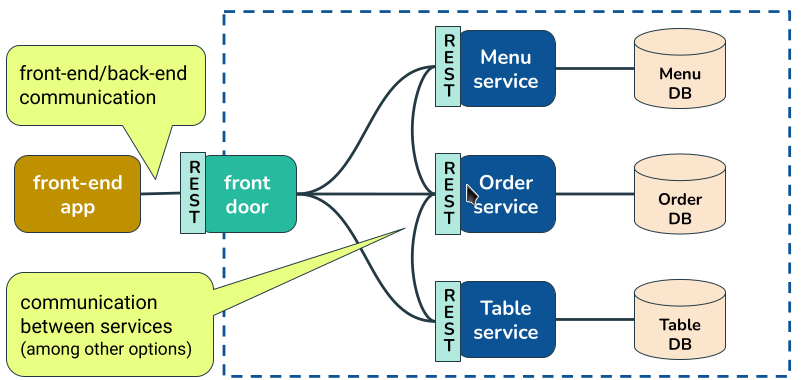
\includegraphics[scale=0.25]{02/msa.png}
	\caption{Utilizzo di REST in MSOAs.}
\end{figure}

\dfn{External Exposed API}{
	API che sono esposte al mondo, Solitamente con un  gateway che blocca l'accesso.
}

\dfn{Internal Service API}{
	API interne all'applicazione con un ingresso.
}

\nt{L'ingresso pubblica quello che esiste, il gateway si occupa di cosa esporre.}

\begin{figure}[h]
	\centering
	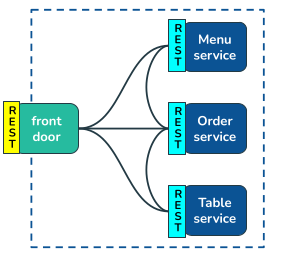
\includegraphics[scale=0.6]{02/API.png}
	\caption{Relazione tra API interne ed esterne.}
\end{figure}

\section{Docker}

\subsection{Introduzione}

Docker nasce per la necessità di avere basso accoppiamento tra servizi nel momento del deploy e in tutta la fase successiva:

\begin{itemize}
	\item Problemi di \fancyglitter{middleware}: legati al "collante" tra i vari servizi.
	\item Le architetture modulari sono interessanti se il loose coupling avviene sia a livello logico che a livello fisico.
\end{itemize}

\paragraph{L'idea delle Virtual Machine:}

\begin{itemize}
	\item Tante macchine virtuali che eseguono applicazioni.
	\item Si faceva per portabilità tra macchine fisiche.
	\item Ma ciò aveva un enorme overhead.
	\item Da questo nasce l'idea dei container e Docker: aree chiuse, mini sistemi operativi "finti" che danno l'illusione alle applicazioni di girare ognuna sul proprio SO. In questo modo si riduce di molto l'overhead.
\end{itemize}

\begin{figure}[h]
	\centering
	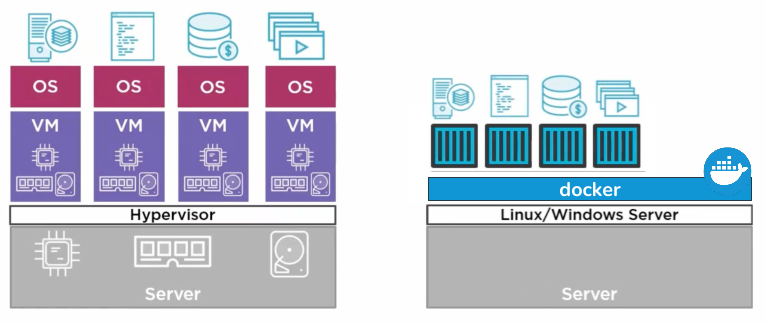
\includegraphics[scale=0.6]{02/vmc.png}
	\caption{Virtual Machine vs. Docker.}
\end{figure}


\dfn{Docker}{
	Docker è un software open-source che utilizza la virtualizzazione a livello di sistema operativo per eseguire applicazioni in ambienti isolati.
}

\subsection{Concetti Importanti}

\dfn{Immagine}{
	Un'immagine è un pacchetto standalone e leggero che include tutto ciò che è necessario per eseguire un'applicazione.
}

\clm{Immagine}{}{
	\begin{itemize}
		\item Sono come dei mini sistemi operativi con le loro specifiche configurazioni e dipendenze.
		\item Le applicazioni "viaggiano" con tutto ciò che serve per poterle eseguire.
		\item Sono parzialmente-portatili: hanno comunque una dipendenza dall'architettura (eccezione per applicazioni java).
		\item Sono fatte da strati (read-only) separati e da un manifest che dice a docker come gli strati dovrebbero essere impilati.
		\item Solo l'ultimo strato è scrivibile.
	\end{itemize}
}

\dfn{Container}{
	Un'istanza in esecuzione di un'immagine Docker.
}

\paragraph{Features di un container:}

\begin{itemize}
	\item \fancyglitter{Leggeri:} non sono macchine virtuali, condividono il kernel del loro OS.
	\item \fancyglitter{Isolati:} ogni container esegue in un envinronment isolato che non interviene con gli altri container.
	\item \fancyglitter{Portabili:} i container non dipendono dal loro host.
	\item \fancyglitter{Effimeri:} possono partire ed essere fermati facilmente.

\end{itemize}

\dfn{Docker Inc.}{
	Docker Inc è la società che fornisce:
	\begin{itemize}
		\item Il Docker engine distribuito sotto Apache 2.0.
		\item Il Docker desktop distribuito per piccoli utenti e aziende sotto licenza GNU.
		\item Docker hub: servizio pubblico di immagini Docker.
	\end{itemize}
}

\begin{figure}[h]
	\centering
	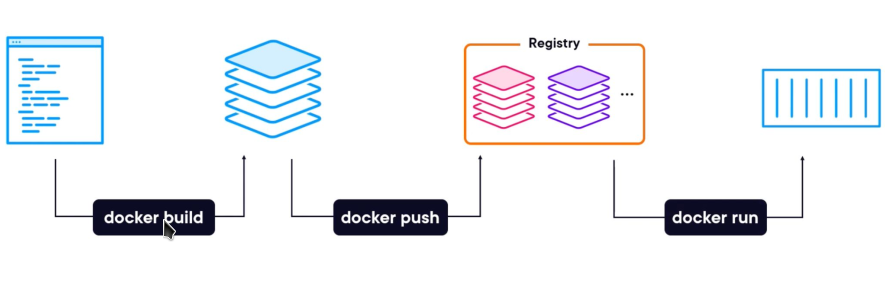
\includegraphics[scale=0.4]{02/dw.png}
	\caption{Docker workflow.}
\end{figure}

\paragraph{Docker workflow:}

\begin{itemize}
	\item build: il progetto viene costruito.
	\item push: su un repository condivido (tipo docker-hub).
	\item run: creazione del container.
\end{itemize}

\subsection{Architettura di Docker}

\begin{figure}[h]
	\centering
	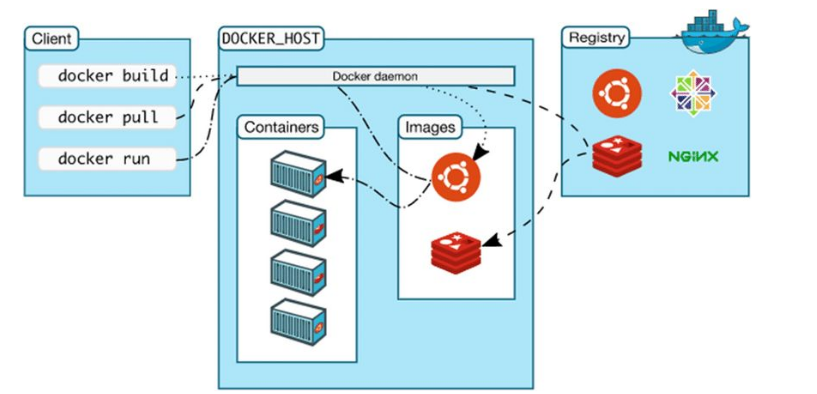
\includegraphics[scale=0.4]{02/arch.png}
	\caption{Architettura di Docker.}
\end{figure}

\paragraph{Architettura:}

\begin{itemize}
	\item Client: per poter eseguire i comandi.
	\item Docker host.
	\item Registry: locale o remoto.
\end{itemize}

\qs{}{Come vengono fatti i conteiners di docker?}

\paragraph{Sfruttando due caratteristiche di linux:}

\begin{itemize}
	\item Control groups: limitano l'accesso alle risorse date a dei gruppi di processi (CPU, RAAM, etc.).
	\item Namespaces: permettono di partizionare le risorse della macchina (id dei processi, filesystem, segmenti di memoria, etc).
\end{itemize}

\paragraph{Volumi persistenti:}

\begin{itemize}
	\item Il filesystem è scrivibile a patto di avere i giusti permessi.
	\item Di base non è peristente.
	\item Per ottenere una completa persistenza si può:
	      \begin{itemize}
		      \item Definire un volume in Docker e mapparlo sul OS.
	      \end{itemize}
\end{itemize}

\subsection{Networking in Docker}

\paragraph{Un container è assimilabile a un computer attaccato alla rete:}

\begin{itemize}
	\item Docker crea una rete virtuale dove i containers sono i nodi.
	\item Ogni container ha un IP.
	\item Al loro interno localhost è 127.0.0.1.
\end{itemize}

\paragraph{Quando un container espone una porta:}

\begin{itemize}
	\item La porta esposta è mappata all'IP internal port del container.
	\item Le richieste vengono ridirette al proprio container.
\end{itemize}

\begin{figure}[h]
	\centering
	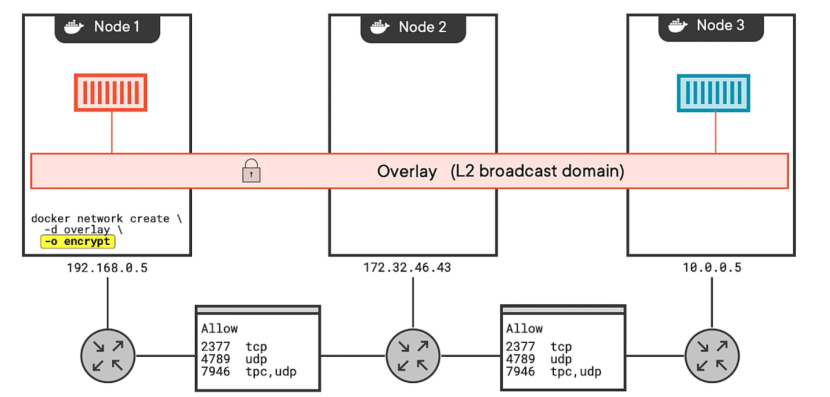
\includegraphics[scale=0.4]{02/over.png}
	\caption{Docker overlay network.}
\end{figure}

\paragraph{Esistono vari tipi di rete:}

\begin{itemize}
	\item Bridge.
	\item IPvlan.
	\item Macvlan.
	\item Overlay.
\end{itemize}

\subsection{Composing Containers}

\dfn{Docker Compose}{
	Sistema per gestire il ciclo di vita di un'applicazione Docker composta da più container.
}

\begin{figure}[h]
	\centering
	
\includegraphics[scale=0.6]{02/compose.png}
	\caption{Docker Compose.}
\end{figure}

\nt{È un unico file yml che specifica tutti i dati necessari per avviare/fermare i servizi.}

\paragraph{Docker workflow:}

\begin{itemize}
	\item build: costruisce le immagini, i volumi e le reti.
	\item up: avvia i servizi.
	\item down: ferma i servizi.
\end{itemize}

\paragraph{Compose:}

\begin{itemize}
	\item È usato per lo sviluppo e i test, non in produzione.
	\item Viene usato per far ripartire i servizi in caso di fallimento.
\end{itemize}
